\documentclass[letterpaper,11pt]{article}
\oddsidemargin -1.0cm \textwidth 17.5cm

\usepackage[utf8]{inputenc}
\usepackage[activeacute,spanish]{babel}
\usepackage{amsfonts,setspace}
\usepackage{amsmath}
\usepackage{amssymb, amsmath, amsthm}
\usepackage{comment}
\usepackage{amssymb}
\usepackage{dsfont}
\usepackage{anysize}
\usepackage{multicol}
\usepackage{enumerate}
\usepackage{graphicx}
\usepackage[left=1.5cm,top=2cm,right=1.5cm, bottom=1.7cm]{geometry}
\setlength\headheight{1.5em} 
\usepackage{fancyhdr}
\usepackage{multicol}
\usepackage{hyperref}
\usepackage{wrapfig}
\usepackage{subcaption}
\pagestyle{fancy}
\fancyhf{}
\renewcommand{\labelenumi}{\normalsize\bfseries P\arabic{enumi}.}
\renewcommand{\labelenumii}{\normalsize\bfseries (\alph{enumii})}
\renewcommand{\labelenumiii}{\normalsize\bfseries \roman{enumiii})}

\begin{document}

\fancyhead[L]{\itshape{Facultad de Ciencias F\'isicas y Matem\'aticas}}
\fancyhead[R]{\itshape{Universidad de Chile}}

\begin{minipage}{11.5cm}
    \begin{flushleft}
        \hspace*{-0.6cm}\textbf{FI1000-5 Introducción a la Física Clásica}\\
        \hspace*{-0.6cm}\textbf{Profesora:} Paulina Lira\\
        \hspace*{-0.6cm}\textbf{Auxiliares:} Alejandro Silva, Felipe Kaschel, Juan Cristóbal Castro\\
    \end{flushleft}
\end{minipage}

\begin{picture}(2,3)
    \put(366,-4){
\includegraphics[scale=0.9]{2020-1/Imágenes/logo/dfi-fcfm.pdf}}
\end{picture}

\begin{center}
	\LARGE \bf Auxiliar Extra C2\\
\end{center}

\vspace{-1cm}
\begin{enumerate}\setlength{\itemsep}{0.4cm}

\rfoot[]{pág. \thepage}

\item[]

\item Considere una superficie horizontal rugosa que empalma suavemente con un tubo semicircular pulido de radio $R$. Un cubo pequeño de masa no nula es lanzado desde $P$ sobre la superficie, ingresa por el tubo y emerge desde su extremo superior hasta caer sobre el punto de partida $P$. La longitud del tramo rugoso es $D$ y el coeficiente de roce cinético con el cubo es $\mu$.
    \begin{enumerate}
        \item Determine la rapidez con la cual debe partir el cubo para que lo descrito sea posible.
        \item Analice e interprete su resultado para el caso $D \sim 0$
    \end{enumerate}

\item Un bloque de masa $M$ con una superficie superior con la forma de medio cilindro de radio ${R}$ se encuentra sobre una superficie horizontal sin rozamiento al tiempo que toca un muro vertical en su lado izquierdo. Una partícula de masa ${m}$ se suelta desde el extremo superior izquierdo de la cavidad como se muestra en la figura. Suponiendo que la fricción puede despreciarse:
    \begin{enumerate}
        \item Determine la rapidez de la partícula al llegar por primera vez a la parte más baja de su trayectoria.
        \item Examine cualitativamente la acción de la fuerza normal del muro sobre el bloque de masa ${M}$ y determine el instante a partir del cual el bloque se desliza a la derecha. Para tiempos posteriores a este, ¿qué principio de conservación utiliza? 
        \item Determine la rapidez máxima que alcanza el bloque en su movimiento después de soltar la masita ${m}$.
    \end{enumerate}

\item Considere una semiesfera de radio $R$ de masa $M$ que se encuentra sobre una superficie horizontal y apoyada contra una pared tal como se muestra en la figura adjunta. El centro de masas de una semiesfera homogénea queda sobre el eje de simetría y a una distancia ${b} = 3 R / 8$ de la base. Suponga que, entre la semiesfera y el suelo el coeficiente de roce estático es $\mu = 3 / 16$, mientras que entre la pared y la semiesfera el roce es nulo.
    \begin{enumerate}
        \item Realice un diagrama de cuerpo libre para la semiesfera.
        \item Encuentre la magnitud y dirección del torque, respecto al punto de apoyo $P$, ejercido por la fuerza de gravedad cuando la semiesfera está ladeada en un ángulo $\beta$.
        \item Encuentre la fuerza de roce entre la semi-esfera y el suelo
        \item Encuentre el ángulo de inclinación mínimo $\beta_{min}$ posible para que la semiesfera no resbale.
    \end{enumerate}
    \begin{figure}[h!]
        \centering
        \begin{subfigure}[t]{5.4cm}
            \centering
            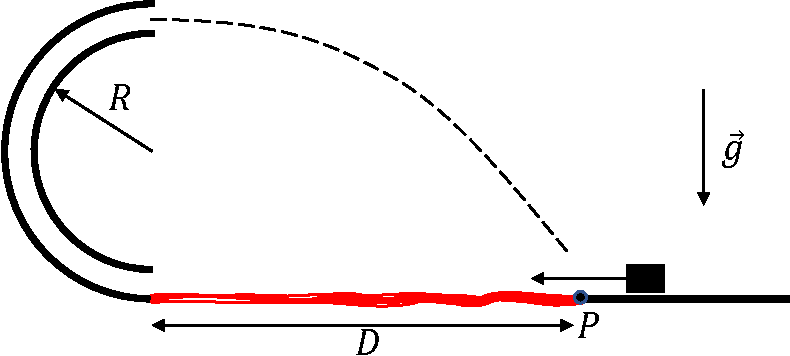
\includegraphics[scale=0.4]{2020-1/Imágenes/aux Extra-C2/p1_extra.pdf}
            \caption*{Figura P1}
        \end{subfigure}
        \qquad 
        \begin{subfigure}[t]{5.4cm}
            \centering
            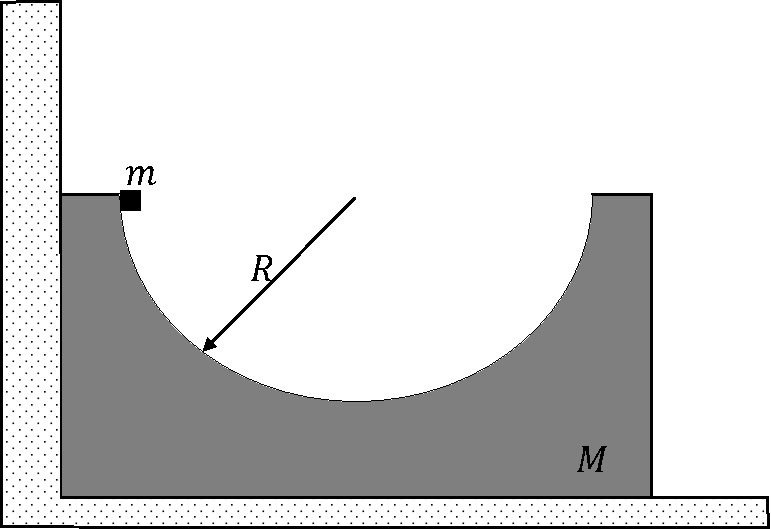
\includegraphics[scale=0.4]{2020-1/Imágenes/aux Extra-C2/p2-extra.pdf}
            \caption*{Figura P2}
        \end{subfigure}
        \begin{subfigure}[t]{5.4cm}
            \centering
            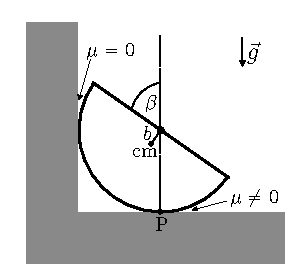
\includegraphics[scale=0.7]{2020-1/Imágenes/aux Extra-C2/semiesfera-torque.pdf}
            \caption*{Figura P3}
        \end{subfigure}
    \end{figure}
\newpage
\item Sea una pieza en forma de círculo de radio $b$ al que le falta un círculo de radio $a$, tal como se muestra en la figura, La masa de la pieza es $M$. Calcule la posición de su centro de masa.

\begin{figure}[h!]
    \centering
    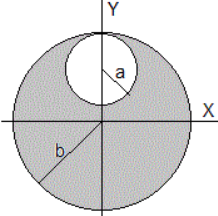
\includegraphics{2020-1/Imágenes/aux Extra-C2/circulo.PNG}
\end{figure}

\item Dos masas $m_1$ y $m_2$, unidos por un resorte de constante $k$, descansan sobre una mesa sin roce. El resorte es comprimido una distancia $d$, con $m_2$ apoyado a una pared y enseguida es abandonado desde el reposo
    \begin{enumerate}
        \item ¿Qué distancia recorre $m_1$ antes que $m_2$ comience a moverse?
        \item En el instante que $m_2$ ha perdido el contacto con la pared, ¿cuál es la velocidad del centro de masa?¿Cuál es la velocidad de cada una de las masas?
    \end{enumerate}
\begin{figure}[h!]
    \centering
    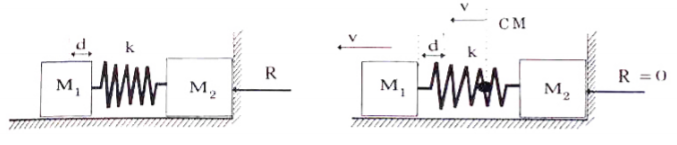
\includegraphics{2020-1/Imágenes/aux Extra-C2/masas-resorte.PNG}
\end{figure}
\end{enumerate}
\end{document}